\documentclass[12pt,a4paper]{article}

\usepackage[utf8]{inputenc}
\usepackage[T1]{fontenc}
\usepackage[french]{babel}
\usepackage{lmodern}
\usepackage{geometry}
\usepackage{graphicx}
\usepackage{booktabs}
\usepackage{float}
\usepackage{amsmath}
\usepackage{longtable}
\usepackage{hyperref}

\geometry{margin=2.5cm}
\graphicspath{{../figures/}}

\begin{document}

% --- DEBUT DE LA PAGE DE GARDE ---
\begin{titlepage}
    \centering
    \vspace*{1cm}

    
\includegraphics[width=0.4\textwidth]{../INSEA_logo.png} \par
    \vspace{2.5cm}

    {\Large \textbf{Module : Séries Chronologiques}}\par
    \vspace{0.5cm}
    {\large Encadré par : Mme Badaoui}\par
    \vspace{2.5cm}

    {\huge \textbf{Application de la méthode de Box-Jenkins}}\par
    \vspace{0.5cm}
    {\Large \textit{Prévision des ventes mensuelles de voitures au Québec}}\par
    \vspace{3cm}

    {\large Réalisé par :}\par
    \vspace{0.5cm}
    \textbf{\Huge \scshape Ait Bargach Ahmed}\par

    \vfill

    {\large Année universitaire 2025--2026}\par
\end{titlepage}

\begin{abstract}
Ce rapport reprend le contenu du notebook \texttt{notebook\_box\_jenkins.ipynb}.
L'objectif est d'appliquer la méthode de Box-Jenkins à la série des ventes
mensuelles de voitures au Québec entre janvier 1960 et décembre 1968. La série est
séparée en un échantillon d'apprentissage, de janvier 1960 à décembre 1966, et un
échantillon de validation, de janvier 1967 à décembre 1968. Après analyse de la
tendance, de la saisonnalité et de la stationnarité, le notebook retient le modèle
SARIMA$(1,1,1)(1,1,1)_{12}$. Sur la période de validation, ce modèle donne une
erreur absolue moyenne de 1191 ventes, une RMSE de 1339 ventes et un MAPE de
5,64 \%, ce qui indique une bonne qualité de prévision.
\end{abstract}

\section{Introduction}

Une série chronologique est une suite d'observations ordonnées dans le temps.
Dans ce projet, on cherche à construire un modèle permettant de prévoir les ventes
mensuelles de voitures. La démarche suivie est celle de Box-Jenkins : visualisation
de la série, séparation apprentissage-validation, analyse qualitative, tests de
stationnarité, étude des corrélogrammes, estimation d'un modèle SARIMA, validation
des résidus et évaluation des prévisions.

Le rapport suit la même organisation que le notebook :
\begin{enumerate}
    \item chargement et visualisation des données ;
    \item division apprentissage / validation ;
    \item analyse qualitative ;
    \item tests de stationnarité ;
    \item corrélogrammes ACF et PACF ;
    \item méthode de Box-Jenkins ;
    \item prévision sur l'échantillon de validation ;
    \item évaluation des performances.
\end{enumerate}

\section{Chargement des données et visualisation}

La série utilisée contient les ventes mensuelles de voitures au Québec entre janvier
1960 et décembre 1968. Elle comporte 108 observations mensuelles. Les données sont
chargées depuis le fichier \texttt{car\_sales.csv}, puis l'indice temporel est
converti en dates mensuelles.

\begin{table}[H]
\centering
\begin{tabular}{lr}
\toprule
Statistique & Valeur \\
\midrule
Nombre d'observations & 108 \\
Moyenne & 15 396 \\
Écart-type & 5 452 \\
Minimum & 6 550 \\
Premier quartile & 11 300 \\
Médiane & 14 494 \\
Troisième quartile & 18 152 \\
Maximum & 29 500 \\
\bottomrule
\end{tabular}
\caption{Statistiques descriptives des ventes mensuelles.}
\end{table}

La figure \ref{fig:serie} montre une tendance croissante sur la période. On observe
aussi des mouvements qui se répètent chaque année, ce qui laisse penser à une
saisonnalité annuelle.

\begin{figure}[H]
\centering
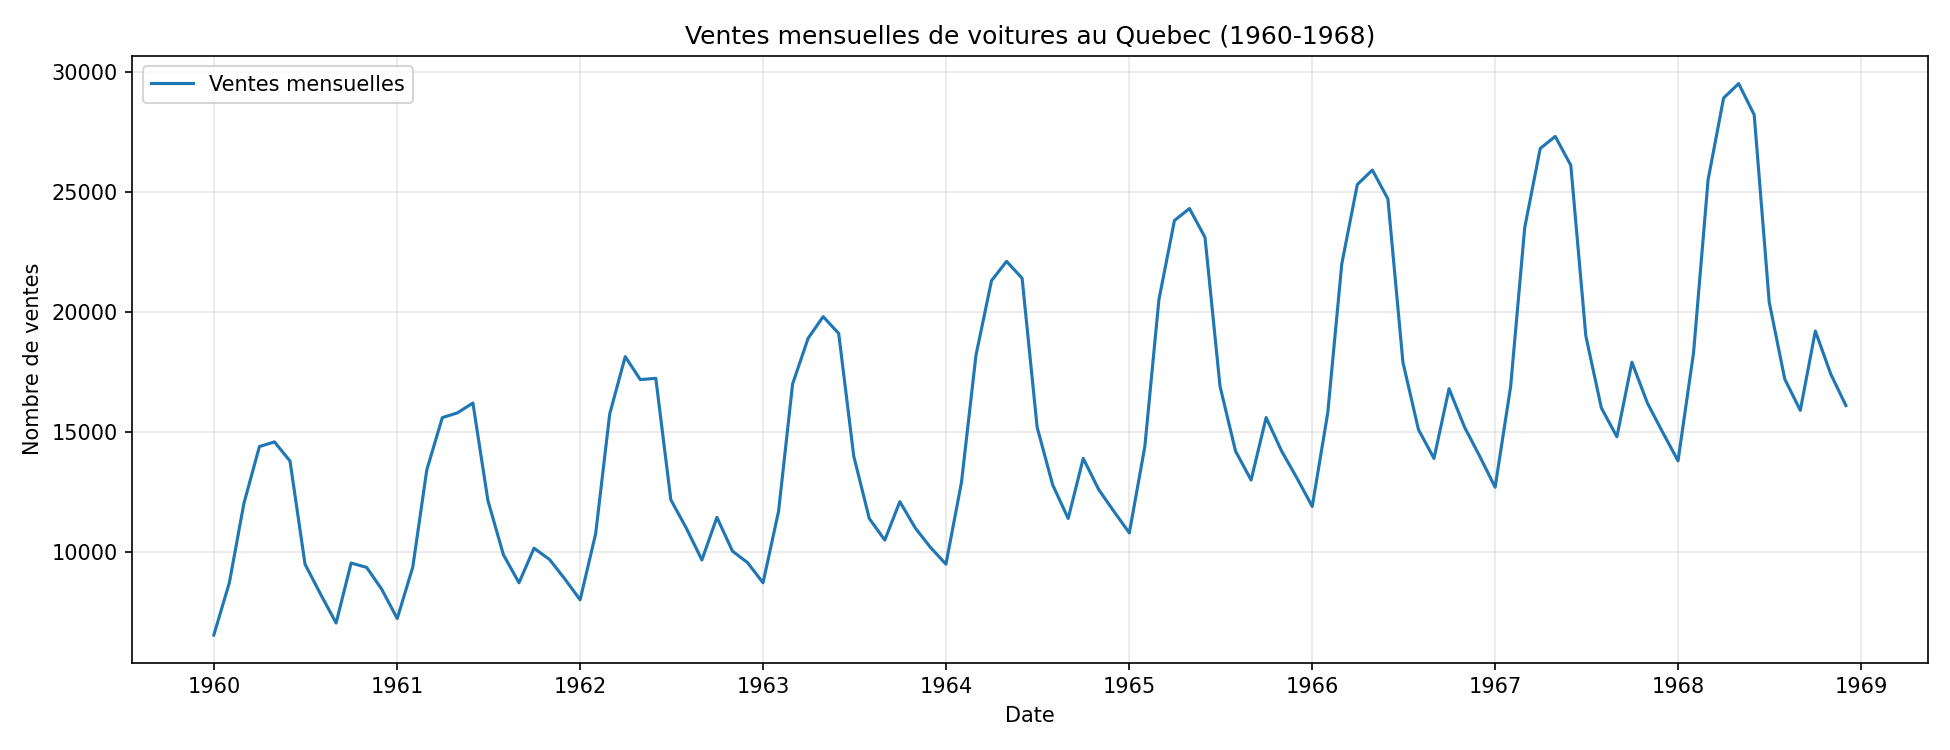
\includegraphics[width=0.92\textwidth]{notebook_serie_complete.png}
\caption{Ventes mensuelles de voitures au Québec entre 1960 et 1968.}
\label{fig:serie}
\end{figure}

\section{Division apprentissage / validation}

Comme dans le notebook, on réserve les 24 dernières observations, soit les deux
dernières années, pour la validation. Le modèle est donc construit sur les données
de janvier 1960 à décembre 1966, puis testé sur les données de janvier 1967 à
décembre 1968.

\begin{table}[H]
\centering
\begin{tabular}{lcc}
\toprule
Échantillon & Période & Taille \\
\midrule
Apprentissage & Janvier 1960 -- Décembre 1966 & 84 \\
Validation & Janvier 1967 -- Décembre 1968 & 24 \\
\bottomrule
\end{tabular}
\caption{Découpage utilisé dans le notebook.}
\end{table}

\begin{figure}[H]
\centering
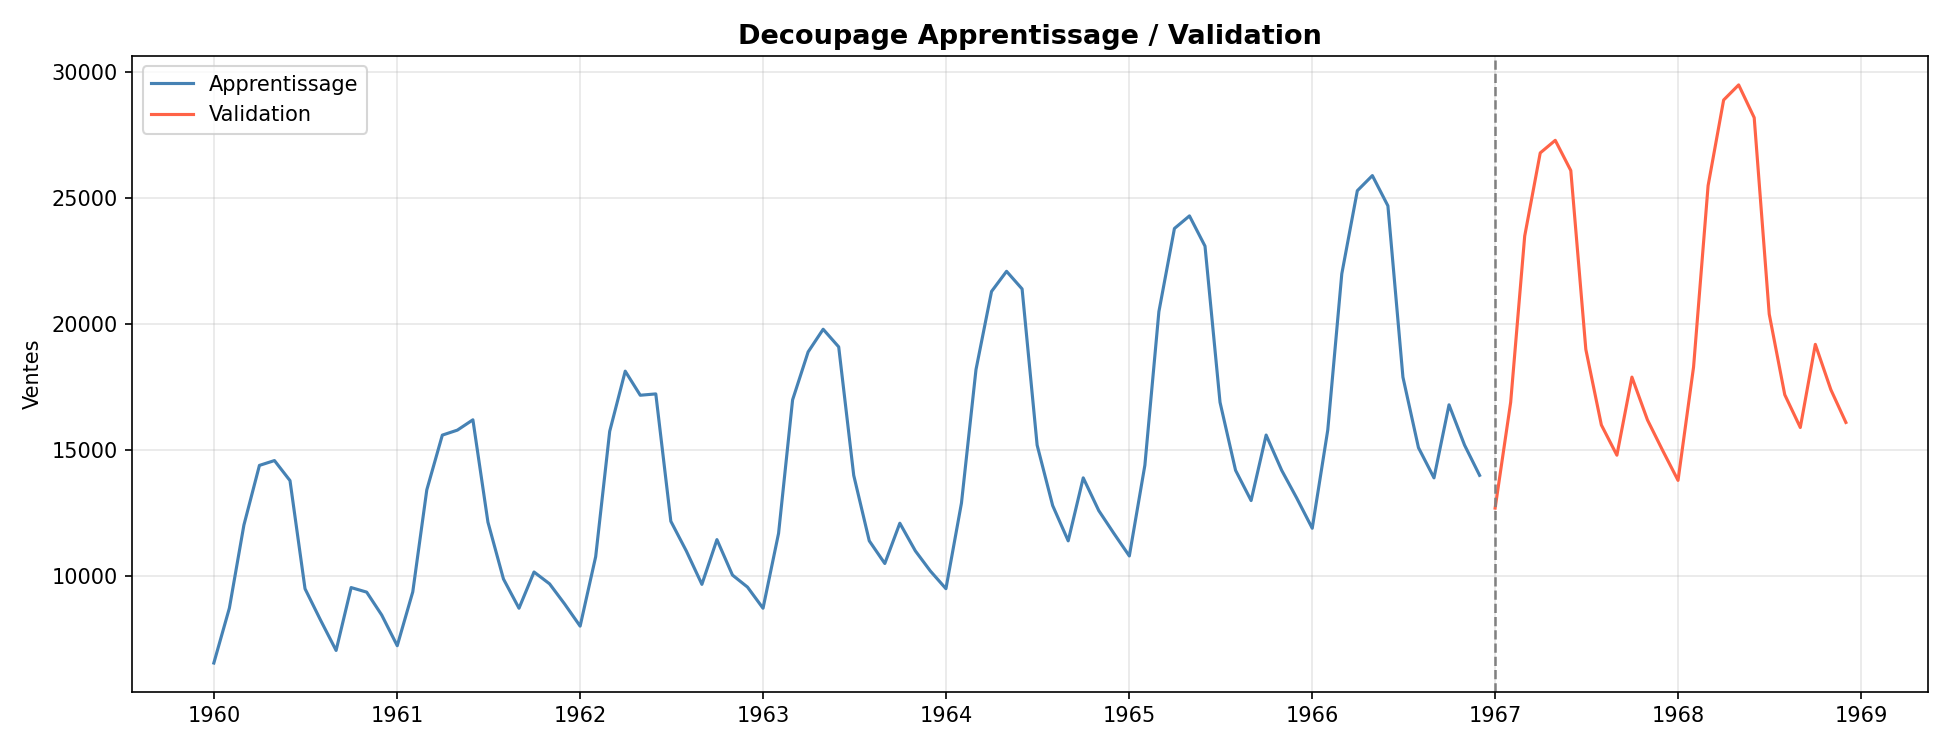
\includegraphics[width=0.92\textwidth]{notebook_split_train_test.png}
\caption{Découpage entre apprentissage et validation.}
\end{figure}

\section{Analyse qualitative de la série}

La décomposition est réalisée sur l'échantillon d'apprentissage. Le notebook utilise
une décomposition multiplicative, car l'amplitude des variations saisonnières
augmente avec le niveau de la série. On considère donc une écriture de la forme :
\[
Y_t = T_t \times S_t \times R_t,
\]
où $T_t$ représente la tendance, $S_t$ la composante saisonnière et $R_t$ le résidu.

\begin{figure}[H]
\centering
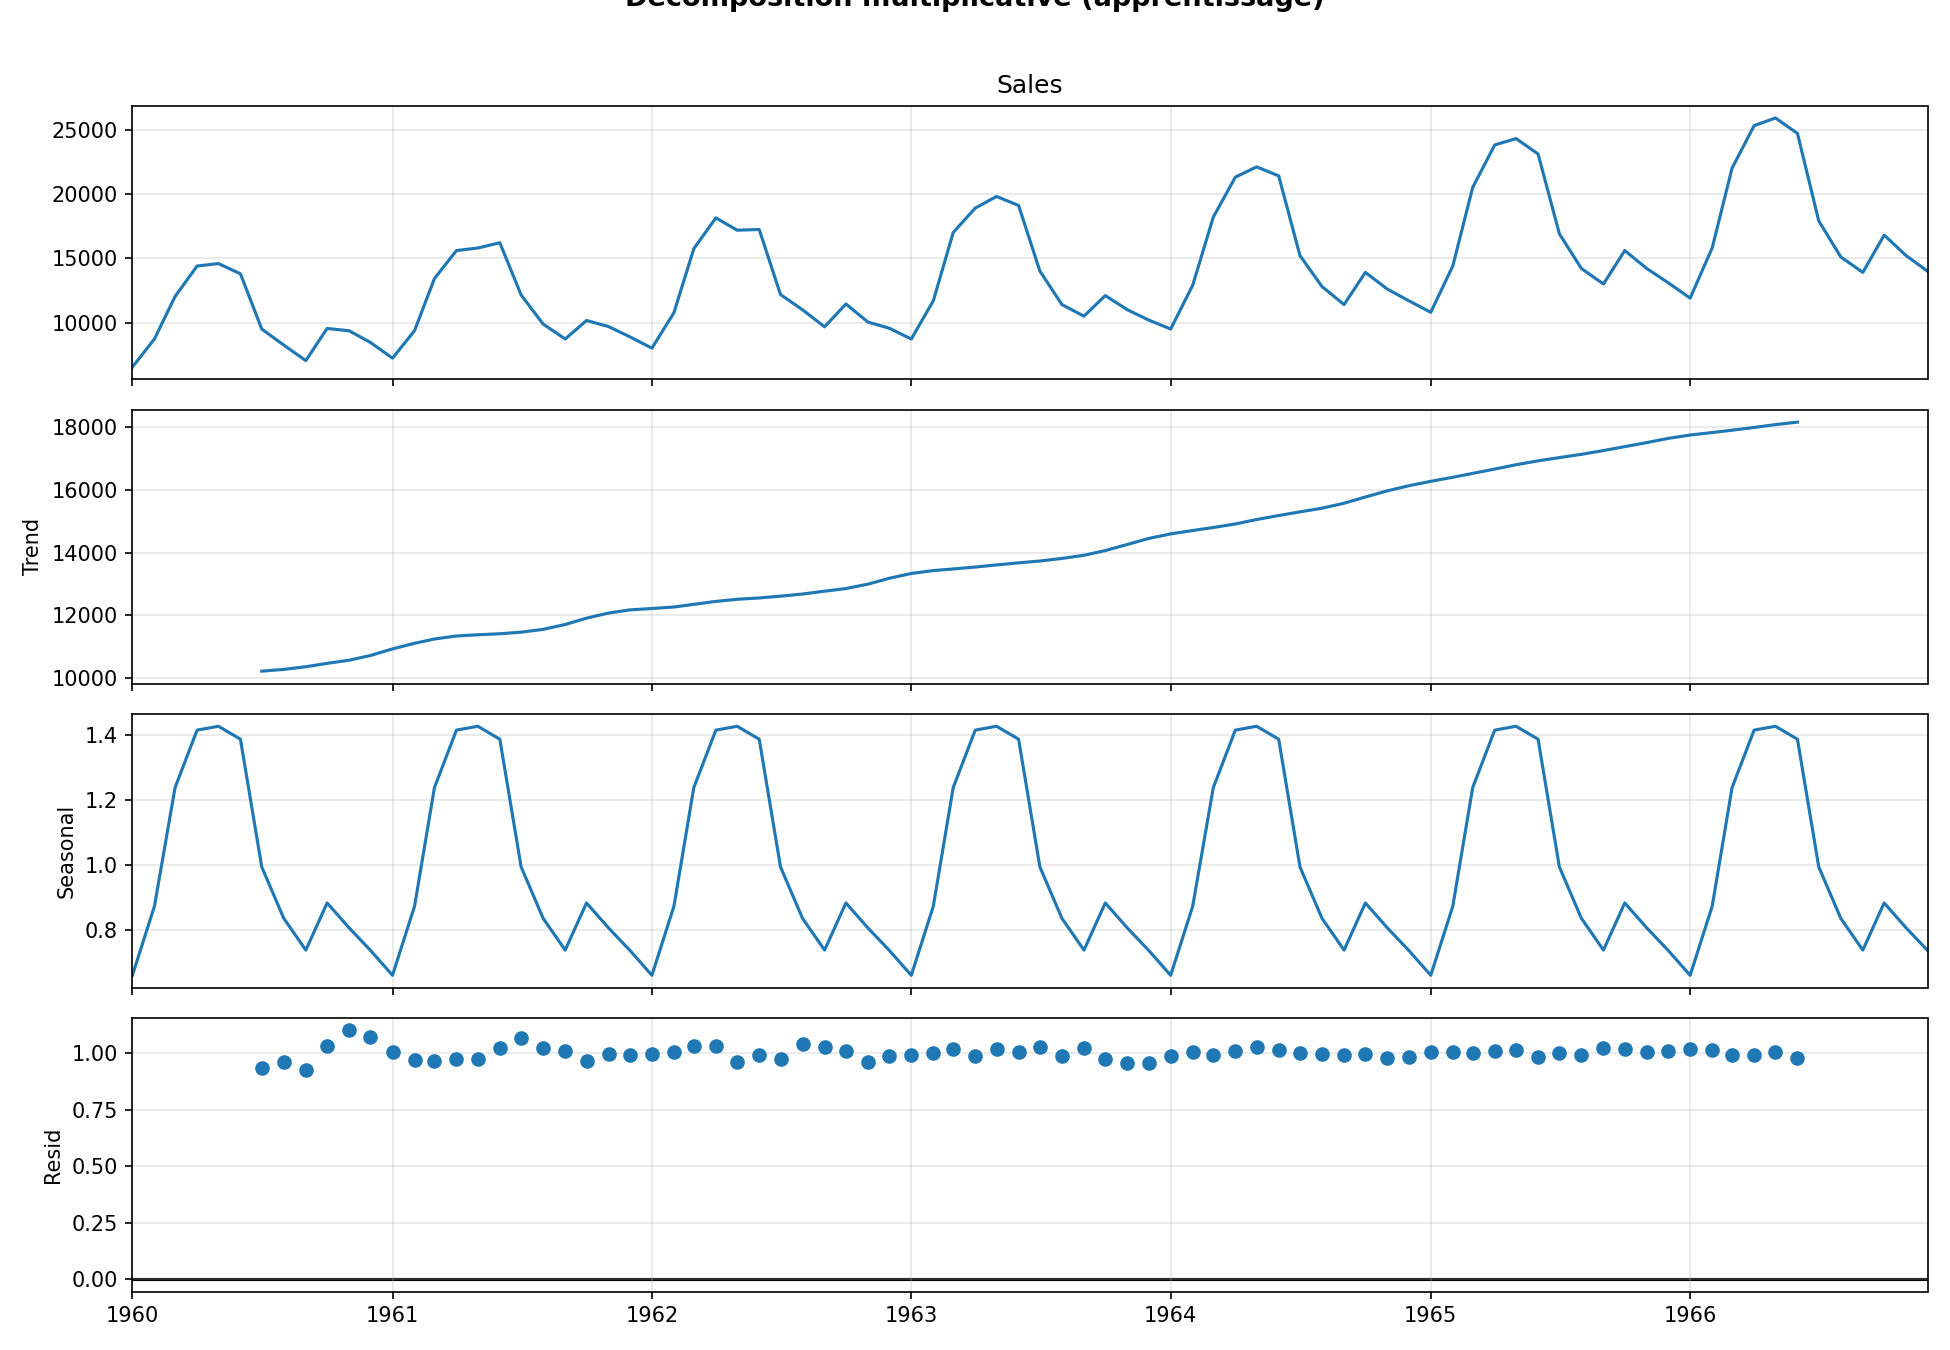
\includegraphics[width=0.92\textwidth]{notebook_decomposition.png}
\caption{Décomposition multiplicative de l'échantillon d'apprentissage.}
\end{figure}

L'interprétation du notebook est la suivante :
\begin{itemize}
    \item la tendance est globalement croissante ;
    \item la saisonnalité est marquée, avec un pic au printemps, surtout en avril-mai ;
    \item le résidu fluctue autour de 1, ce qui est cohérent avec une décomposition multiplicative.
\end{itemize}

La visualisation par mois confirme cette saisonnalité. Les ventes sont plus fortes au
printemps et diminuent généralement au début de l'année et vers la fin de l'année.

\begin{figure}[H]
\centering
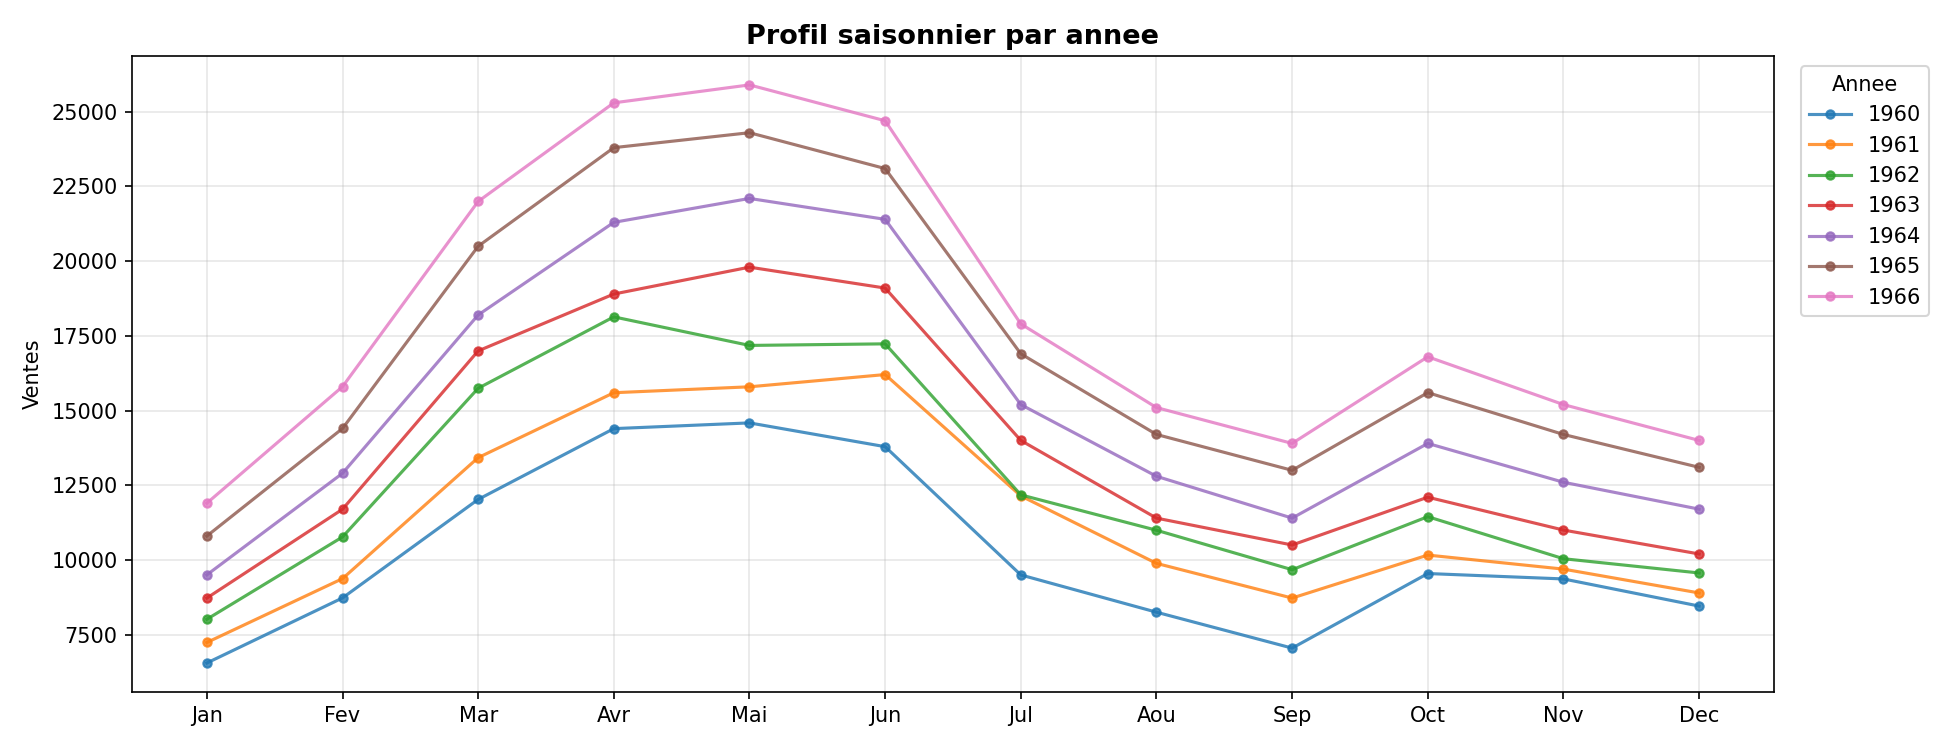
\includegraphics[width=0.92\textwidth]{notebook_saisonnalite.png}
\caption{Profil saisonnier par année.}
\end{figure}

\section{Test de stationnarité}

Le notebook applique deux tests :
\begin{itemize}
    \item le test ADF, dont l'hypothèse nulle est la non-stationnarité ;
    \item le test KPSS, dont l'hypothèse nulle est la stationnarité.
\end{itemize}

La série brute n'est pas stationnaire. La transformation logarithmique seule ne suffit
pas. Après différenciation ordinaire, la série devient stationnaire selon les deux
tests. Le notebook garde aussi la différenciation saisonnière afin de construire un
modèle SARIMA avec $d=1$, $D=1$ et une période saisonnière $s=12$.

\begin{table}[H]
\centering
\begin{tabular}{lcc}
\toprule
Série testée & p-value ADF & p-value KPSS \\
\midrule
Série brute & 0,9886 & 0,0100 \\
$\log(Y_t)$ & 0,7168 & 0,0100 \\
$\Delta \log(Y_t)$ & 0,0002 & 0,1000 \\
$\Delta_{12} \log(Y_t)$ & 0,3437 & 0,1000 \\
$\Delta \Delta_{12} \log(Y_t)$ & 0,0089 & 0,1000 \\
\bottomrule
\end{tabular}
\caption{Tests ADF et KPSS réalisés dans le notebook.}
\end{table}

\begin{figure}[H]
\centering
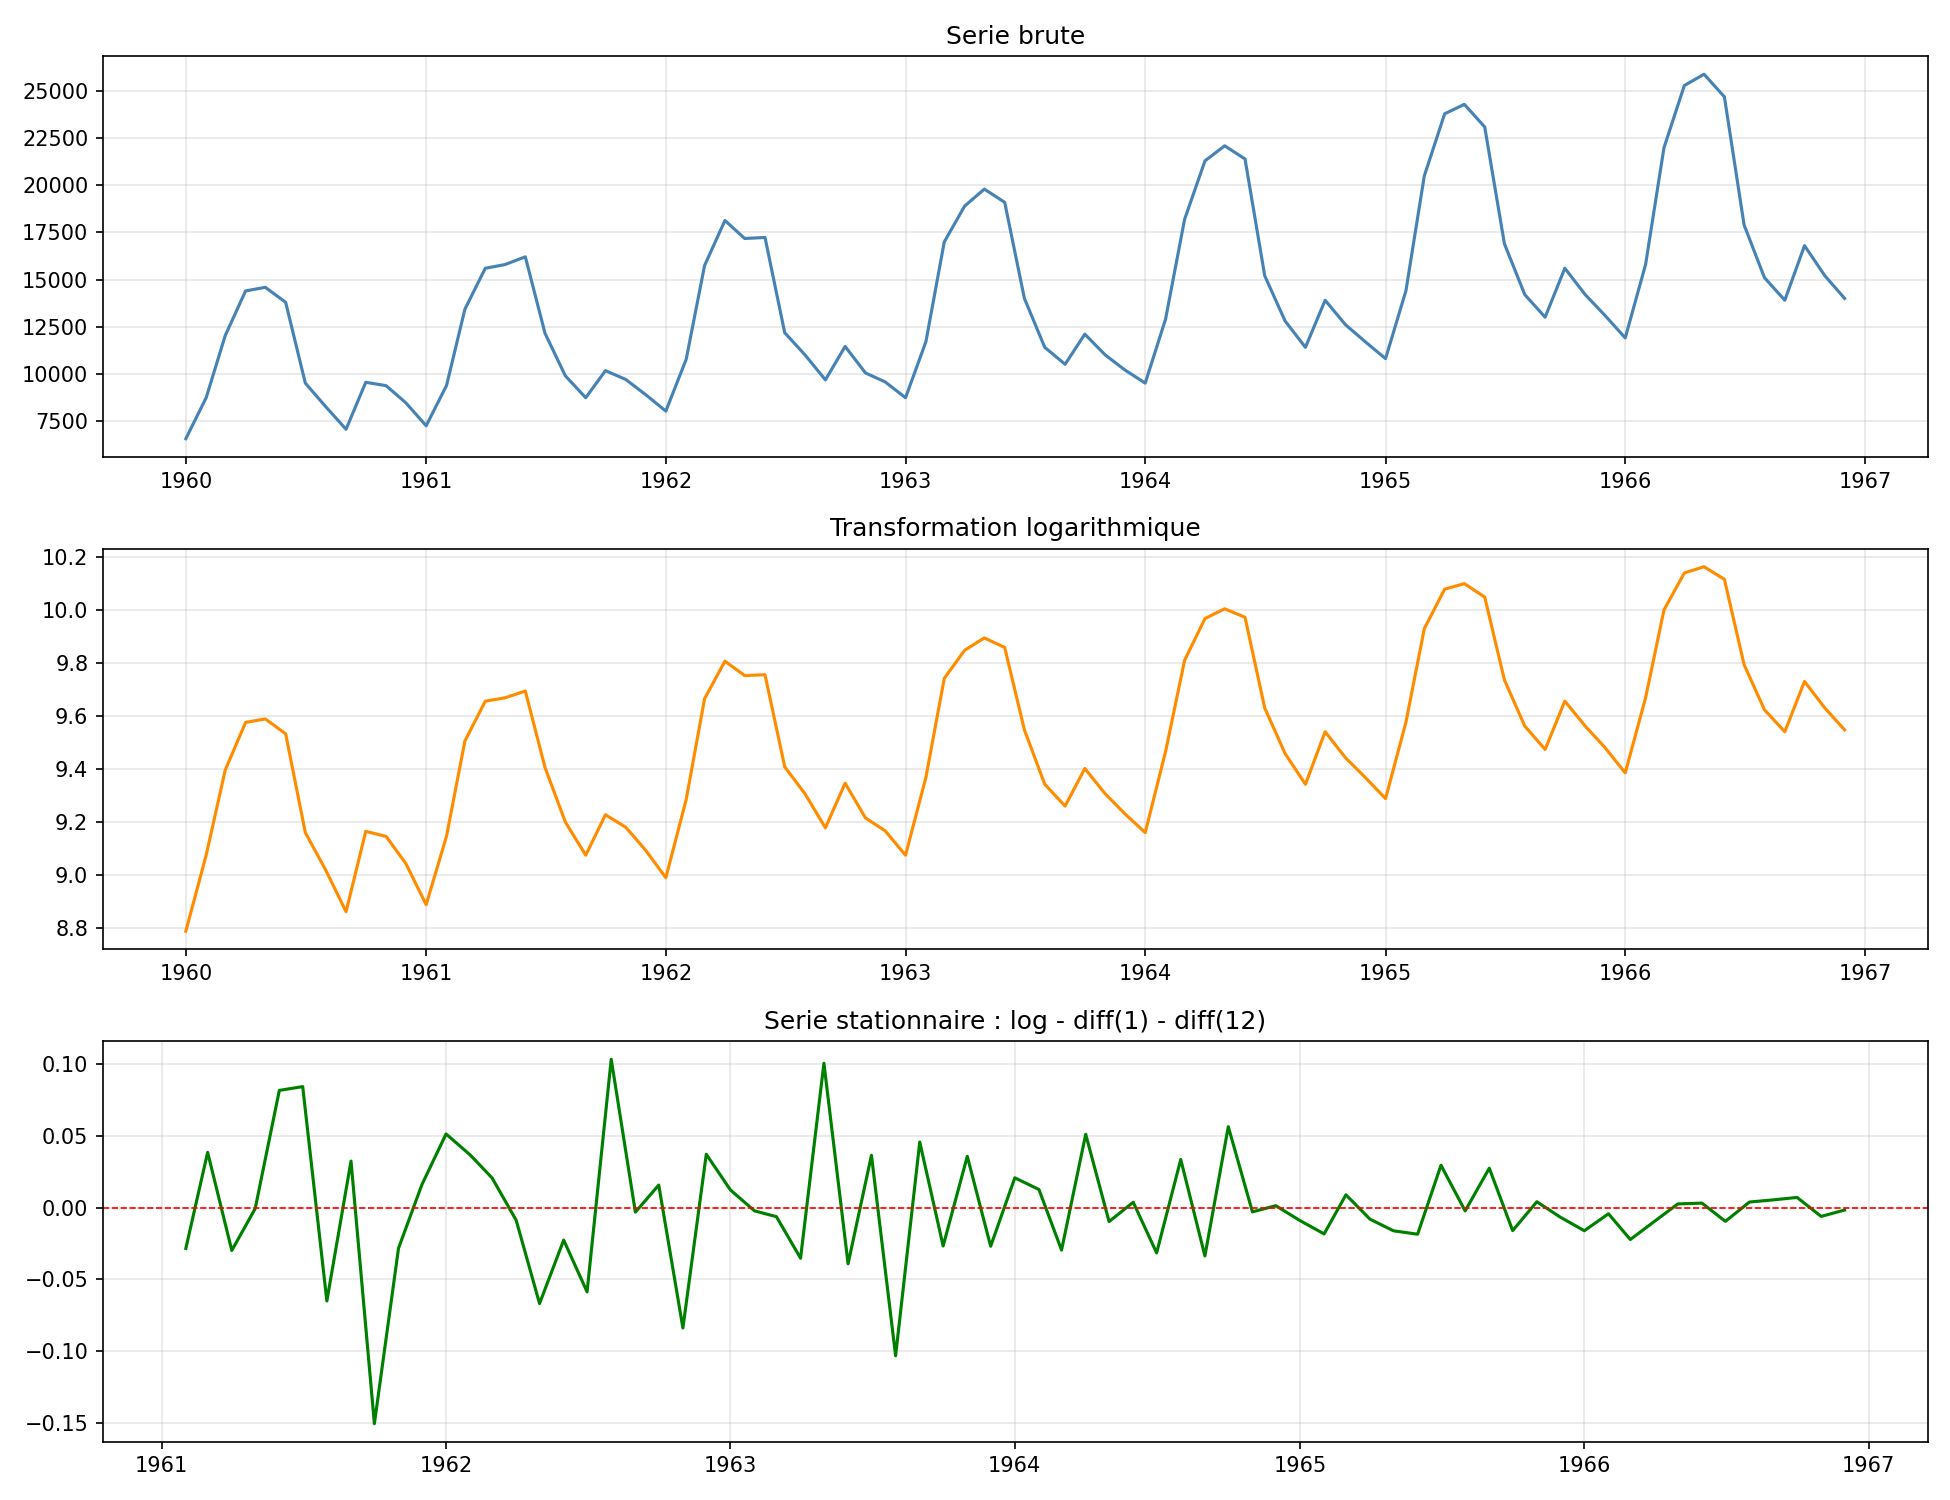
\includegraphics[width=0.92\textwidth]{notebook_transformations.png}
\caption{Série brute, logarithme et série stationnaire.}
\end{figure}

\section{Corrélogrammes ACF et PACF}

Les corrélogrammes sont tracés sur la série stationnaire. Le notebook utilise les
retards jusqu'à 40 pour l'ACF et jusqu'à 30 pour la PACF, ce qui respecte la consigne
d'avoir un décalage d'ordre au moins égal à 36 pour l'ACF.

La lecture proposée est la suivante : l'ACF et la PACF indiquent la présence de
composantes autorégressives et moyenne mobile. Les pics aux retards 12 et 24
confirment la saisonnalité annuelle.

\begin{figure}[H]
\centering
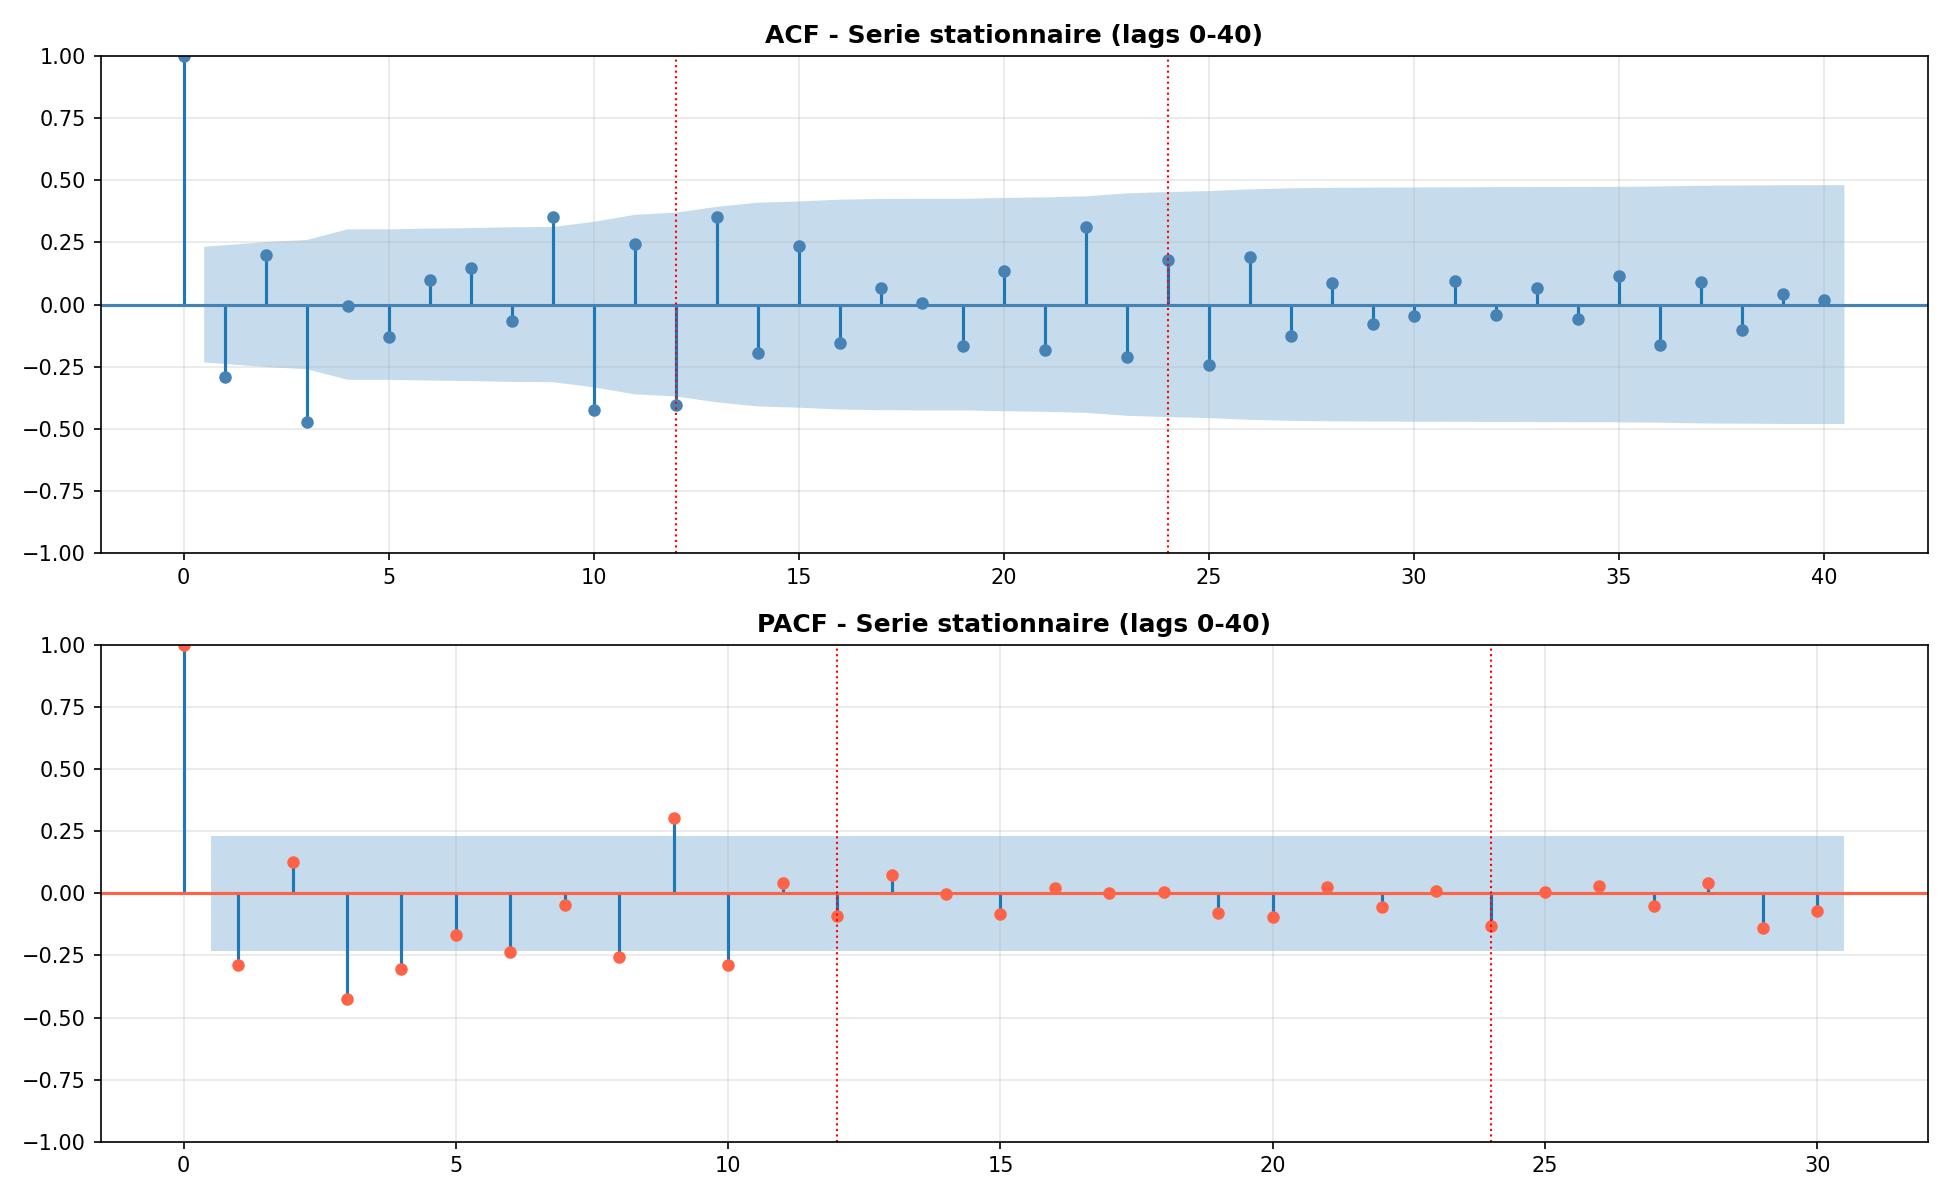
\includegraphics[width=0.92\textwidth]{notebook_acf_pacf.png}
\caption{Corrélogrammes ACF et PACF de la série stationnaire.}
\end{figure}

\section{Méthode de Box-Jenkins : modèle SARIMA}

La série présente une saisonnalité de période 12. Le notebook cherche donc un modèle :
\[
SARIMA(p,1,q)(P,1,Q)_{12}.
\]

Les ordres sont testés sur une petite grille :
\[
p,q \in \{0,1,2\}, \qquad P,Q \in \{0,1\}.
\]
Le critère de sélection utilisé est l'AIC. Le meilleur modèle obtenu dans le notebook
est :
\[
SARIMA(1,1,1)(1,1,1)_{12},
\]
avec un AIC de $-248,98$.

\begin{table}[H]
\centering
\begin{tabular}{lrrrrrrr}
\toprule
Rang & $p$ & $d$ & $q$ & $P$ & $D$ & $Q$ & AIC \\
\midrule
1 & 1 & 1 & 1 & 1 & 1 & 1 & -248,98 \\
2 & 0 & 1 & 2 & 1 & 1 & 0 & -248,81 \\
3 & 2 & 1 & 2 & 0 & 1 & 0 & -248,57 \\
4 & 1 & 1 & 0 & 0 & 1 & 0 & -248,11 \\
5 & 1 & 1 & 2 & 0 & 1 & 0 & -247,36 \\
\bottomrule
\end{tabular}
\caption{Cinq meilleurs modèles selon l'AIC.}
\end{table}

Le modèle retenu peut s'écrire, sur la série logarithmique :
\[
(1-\phi_1B)(1-\Phi_1B^{12})(1-B)(1-B^{12})\log(Y_t)
= (1+\theta_1B)(1+\Theta_1B^{12})\varepsilon_t.
\]

\section{Validation des résidus}

Après estimation, le notebook trace les diagnostics des résidus. L'objectif est de
vérifier que les résidus ressemblent à un bruit blanc : pas de structure visible,
histogramme raisonnablement centré, QQ-plot proche de la diagonale et ACF des résidus
sans pics importants.

\begin{figure}[H]
\centering
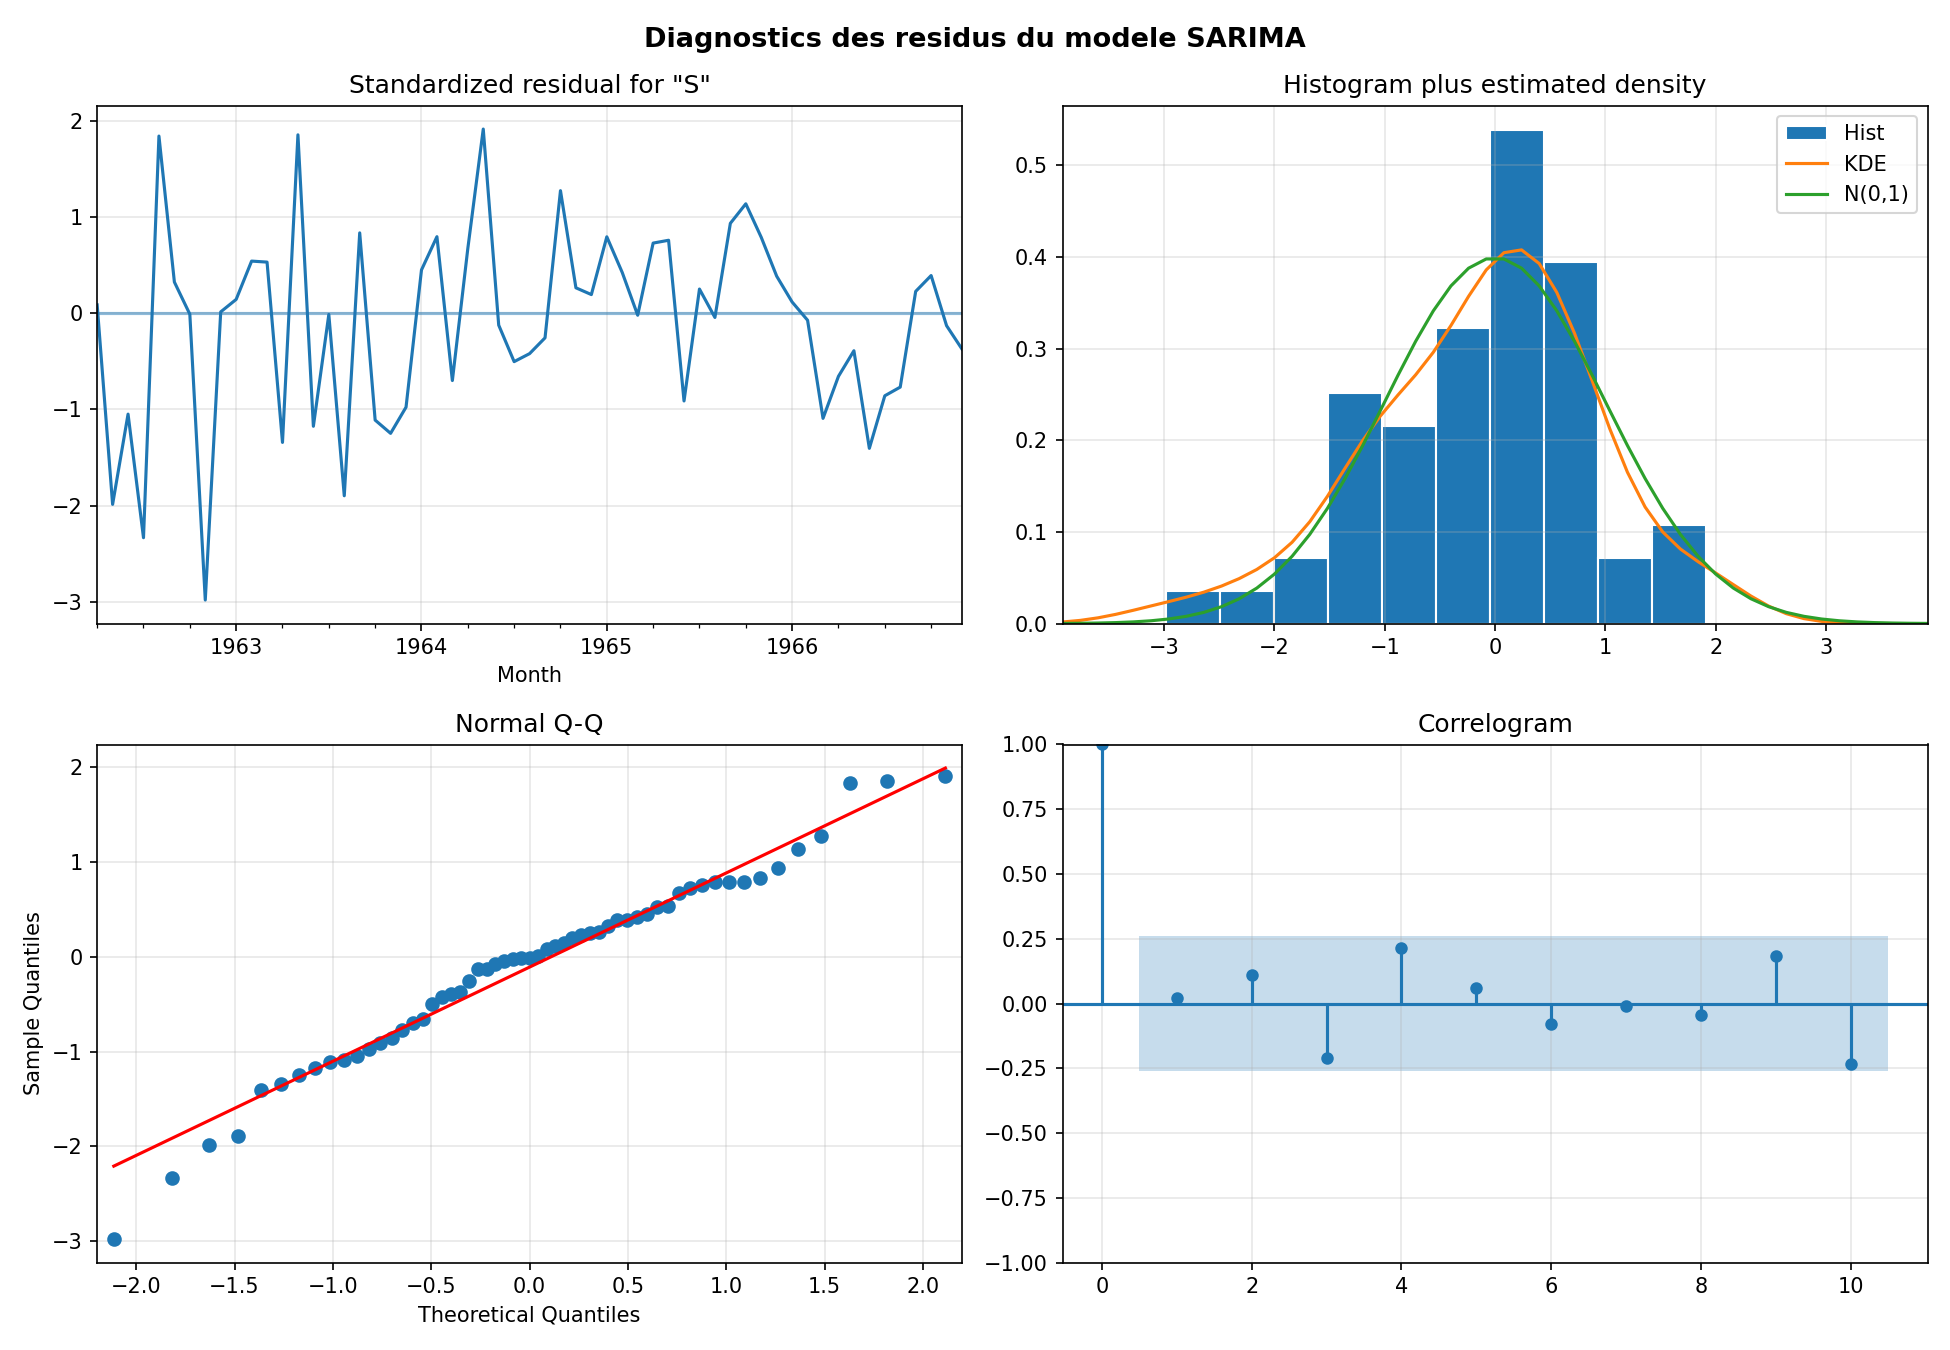
\includegraphics[width=0.92\textwidth]{notebook_diagnostics_residus.png}
\caption{Diagnostics des résidus du modèle SARIMA retenu.}
\end{figure}

\section{Prévision sur l'échantillon de validation}

Le modèle SARIMA$(1,1,1)(1,1,1)_{12}$ est ensuite utilisé pour prévoir les 24 mois de
l'échantillon de validation. Les prévisions sont obtenues sur l'échelle logarithmique,
puis transformées avec l'exponentielle pour revenir à l'échelle initiale des ventes.

\begin{figure}[H]
\centering
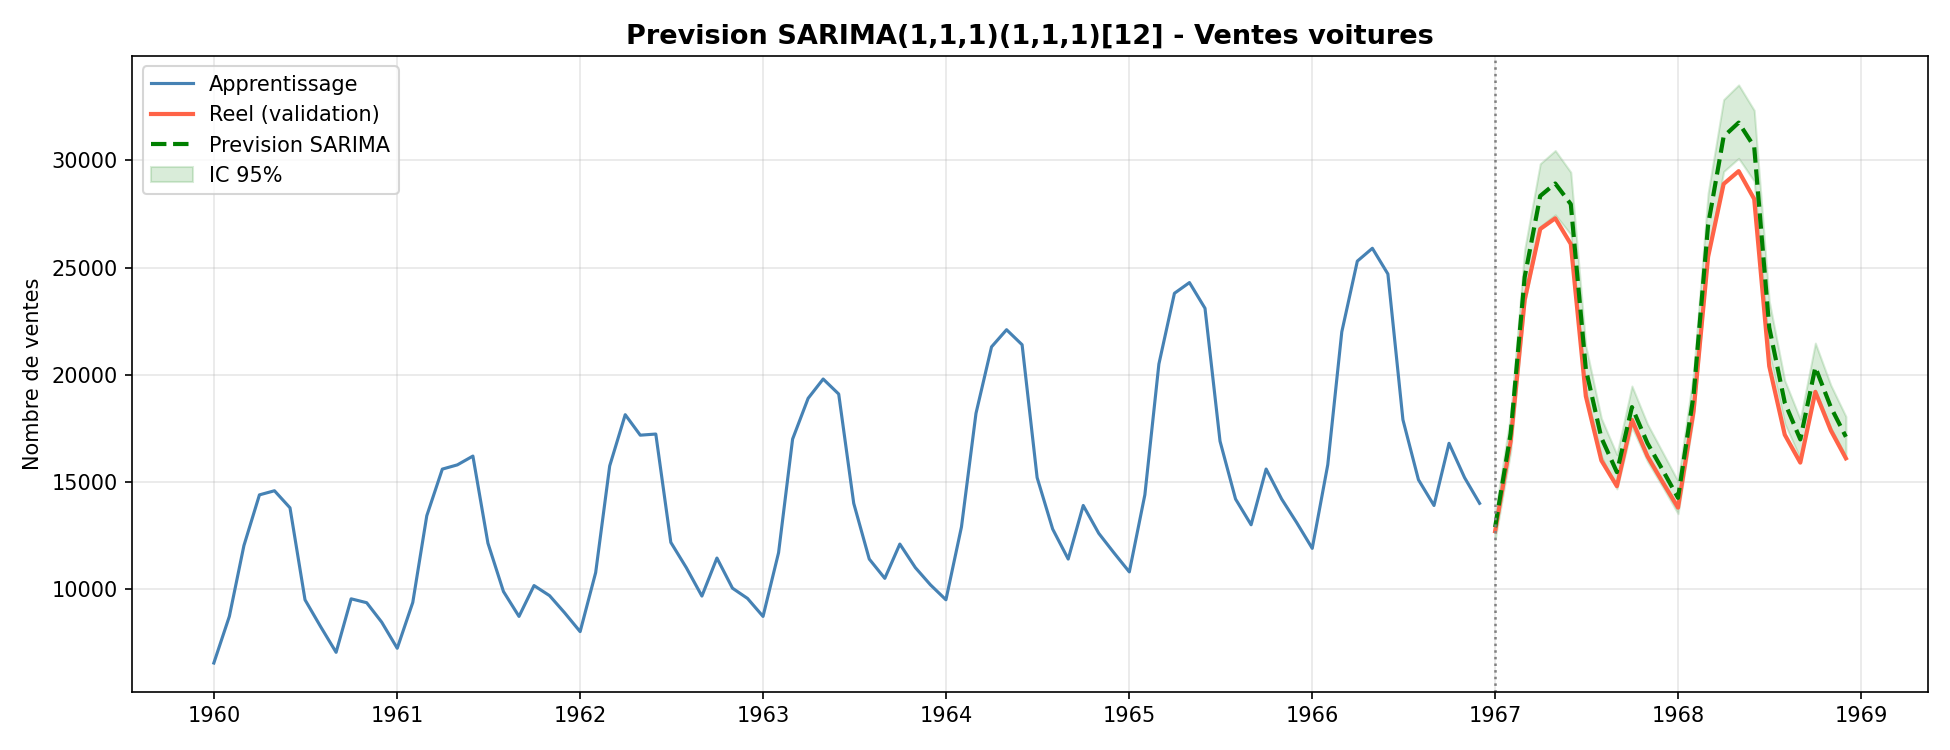
\includegraphics[width=0.92\textwidth]{notebook_prevision.png}
\caption{Prévision SARIMA sur l'échantillon de validation.}
\end{figure}

\section{Évaluation des performances}

Les indicateurs utilisés sont :
\[
MAE = \frac{1}{n}\sum_{t=1}^{n}|Y_t-\widehat{Y}_t|,
\]
\[
RMSE = \sqrt{\frac{1}{n}\sum_{t=1}^{n}(Y_t-\widehat{Y}_t)^2},
\]
\[
MAPE = \frac{100}{n}\sum_{t=1}^{n}\left|\frac{Y_t-\widehat{Y}_t}{Y_t}\right|.
\]

Sur l'échantillon de validation, le notebook obtient :

\begin{table}[H]
\centering
\begin{tabular}{lr}
\toprule
Indicateur & Valeur \\
\midrule
MAE & 1 191 \\
RMSE & 1 339 \\
MAPE & 5,64 \% \\
\bottomrule
\end{tabular}
\caption{Performance du modèle sur la validation.}
\end{table}

Comme le MAPE est inférieur à 10 \%, le notebook conclut que la prévision est
excellente selon ce critère.

\begin{table}[H]
\centering
\scriptsize
\resizebox{\textwidth}{!}{%
\begin{tabular}{lrrrr}
\toprule
Date & Réel & Prévision & Erreur abs. & Erreur (\%) \\
\midrule
Jan 1967 & 12 700 & 12 890 & 190 & 1,49 \\
Fév 1967 & 16 900 & 17 255 & 355 & 2,10 \\
Mar 1967 & 23 500 & 24 559 & 1 059 & 4,50 \\
Avr 1967 & 26 800 & 28 342 & 1 542 & 5,75 \\
Mai 1967 & 27 300 & 28 922 & 1 622 & 5,94 \\
Juin 1967 & 26 100 & 27 960 & 1 860 & 7,13 \\
Juil 1967 & 19 000 & 20 265 & 1 265 & 6,66 \\
Août 1967 & 16 000 & 17 058 & 1 058 & 6,61 \\
Sep 1967 & 14 800 & 15 454 & 654 & 4,42 \\
Oct 1967 & 17 900 & 18 490 & 590 & 3,30 \\
Nov 1967 & 16 200 & 16 807 & 607 & 3,74 \\
Déc 1967 & 15 000 & 15 565 & 565 & 3,77 \\
Jan 1968 & 13 800 & 14 256 & 456 & 3,30 \\
Fév 1968 & 18 300 & 19 034 & 734 & 4,01 \\
Mar 1968 & 25 500 & 26 982 & 1 482 & 5,81 \\
Avr 1968 & 28 900 & 31 114 & 2 214 & 7,66 \\
Mai 1968 & 29 500 & 31 763 & 2 263 & 7,67 \\
Juin 1968 & 28 200 & 30 640 & 2 440 & 8,65 \\
Juil 1968 & 20 400 & 22 206 & 1 806 & 8,85 \\
Août 1968 & 17 200 & 18 699 & 1 499 & 8,71 \\
Sep 1968 & 15 900 & 16 983 & 1 083 & 6,81 \\
Oct 1968 & 19 200 & 20 351 & 1 151 & 5,99 \\
Nov 1968 & 17 400 & 18 485 & 1 085 & 6,23 \\
Déc 1968 & 16 100 & 17 105 & 1 005 & 6,24 \\
\bottomrule
\end{tabular}}
\caption{Valeurs réelles et prévisions sur l'échantillon de validation.}
\end{table}

\section{Conclusion}

Le notebook montre que la série des ventes de voitures possède une tendance croissante
et une saisonnalité annuelle marquée. La transformation logarithmique permet de
stabiliser l'amplitude des variations, puis les différenciations ordinaire et
saisonnière permettent de travailler avec une série stationnaire. La recherche par AIC
retient le modèle SARIMA$(1,1,1)(1,1,1)_{12}$.

Sur les deux années gardées pour la validation, le modèle donne un MAPE de 5,64 \%.
Les prévisions suivent correctement le profil saisonnier de la série. Le modèle est
donc acceptable pour une présentation de niveau ingénieur : il est cohérent avec la
méthode de Box-Jenkins, il respecte les étapes de l'énoncé et il donne une qualité de
prévision satisfaisante.

\end{document}
